\begin{itemize}
    \item IMP hosts systems for identity management and provides access to users with an application and to service providers with integration tools
    \item Users can create an identity and manage attributes (key-value pairs)
    \item Users and service providers can establish relationships and use them to securely share personal information and exchange structured data
\end{itemize}

\begin{itemize}
    \item Ease of Use: Users only need to manage one online identity which can be accessed by multiple service providers
    \item Data protection: Users can control which service providers get access to which attributes
    \item Bidirectional Communication: Service providers and users can directly communicate with each other by exchanging structured data their tools have a common understanding of.
    \item User Interaction: The user application can display various user interfaces based on the content of exchanged structured data.
    \item Data Abuse Protection: Service providers are only supplied with necessary personal information which minimizes the possibilities of abuse by the service provider or in case of a data breach.
    \item Communication Security: Attributes communicated structured data are securely exchanged. User and service provider can therefore also directly exchange sensible information. This is not possible for example through e-mail
\end{itemize}


The purpose of the following sections is not to give a detailed explanation of the presented IMP system but to deliver a brought understanding of the concepts, features and components involved.

\subsection{Features}

\paragraph{Provisioning} The IMP system is hosted on the system architecture of the identity management provider and provides identity management as a service for users and SPs. Users and service providers can manage identities by accessing features of the IMP system. The IMP system stores all personal information and data necessary for the operation of identity management. The user only manages one identity which can be accessed by multiple service providers.

\paragraph{Applications} The IMP system provides users and service providers with software tools for accessing its features. The user is provided with a user friendly application while the enterprise is provided with tools for integration.

\paragraph{Personal Information Management} One feature of the IMP system is management of personal information. Through the application, the user can create an identity and add, remove and update any kind of key-value pairs. These are IMP identity attributes.

\paragraph{Relationship} 

Users and service providers can establish relationships which enables them to share information and interact. The initial form of a relationship is a relationship template. The template is created by the service provider and describes which relationships he is willing to establish. Relationship templates are distributed to interested users which can use it to request relationships. A service provider has to fill a relationship template with some minimal required and some optional information:

\begin{itemize}
    \item \textbf{Title}
    
    The title describes the purpose of the relationship in a short way.
    
    \item \textbf{Requested Attributes} (optional)
    
    Requested Attributes is a list of attribute keys, the user will have to submit as part of the relationship request.
    
    \item \textbf{Shared Attributes}
    
    Shared Attributes is a list of attribute keys and values, the service provider wakes available to any user interested in requesting this relationship. The service provider has to share a minimal amount of attributes which enable the user to identify it. 
    
    \item \textbf{Purpose}
    
    The purpose describes why the user and the service provider want to establish the relationship and why the attributes requested by the user are necessary for it.
    
    \item \textbf{Attachments}
    
    Attachments are documents attached to the relationship template by the service provider. The documents can for example contain legal information.
    
    \item \textbf{Metadata}
    
    Metadata can be any type of information which should not be displayed to the user but is necessary for the user application or the service provider to process the resulting relationship request.
    
\end{itemize}

When the user receives the template through his IMP tooling, the requested attributes are automatically filled in if he previously added them to his IMP identity. Otherwise he can fill in the correct values now and automatically add them as attributes of his identity.

It is important to differentiate identity attributes from the attributes shared as part of the relationship. Identity attributes are managed by the user to reflect the most up to date information. Attributes shared as part of a relationship can be automatically filled with values from the same attributes of the IMP identity but can also be manually entered. This means, shared attributes and IMP identity attributes are not necessarily the same.

Based on the information about the service provider and the purpose of the relationship, the user can decide to send a relationship request or not. If the user decides to request the relationship, the request is sent to the service provider along with a copy of the requested attributes. If the service provider approves the request, the relationship is established and both parties get notified.

\paragraph{Messages} As part of a relationship, user and service provider can interact with each other by asynchronously exchanging structured data (IMP messages). Messages with any content can be exchanged, however, the tools used by the user and the service provider should be able to understand the messages.

The integration tool for the service provider does not understand the content of messages but simply makes the accessible by the system architecture of the service provider. Without additional integration solutions, the service provider has to implement his own solutions for processing the different types of messages. The application provided to the user has a set of messages it understands. The list of messages the application is able to process can be expanded by the identity management provider who develops it.

Some important messages the user application understands and the service provider should be able to process too are:

\begin{itemize}
    \item \textbf{Mails}
    
    Mails are messages which contain a human readable title, and body.
    
    \item \textbf{Attribute Change}
    
    After a relationship is established, service provider or user might want to change attributes they shared. This can be done by exchanging request-reply messages.
\end{itemize}

\paragraph{Security}
The IMP system guarantees, that all information is encrypted and can only be decrypted by identities which are allowed to read it. Only the owner of an identity can manage attributes of his identity. A relationship is established only with the identity presented as part of the relationship request and only the specified attributes are shared. Interactions as part of a relationship are only possible between the identities of the relationship. 

\subsection{Evaluation of Features}

This section evaluates the advantages and disadvantages of the described features of the IMP system based on the requirements of users and service providers.

\subsubsection{User}
The IMP system enables users to manage one identity and share attributes with multiple service providers. This replaces the need of a user profile for all service providers which take advantage of the IMP service. The user wont have to access multiple websites for managing user profiles but update his identity only through the IMP service.
As attributes can only be shared with service providers as part of a relationship, the user has control of his personal information. Before accepting the relationship, he can see information about the identity of the service provider, like his name, address, phone number and more. The user is also provided with information on why the relationship and request attributes are necessary which helps the user in deciding if he agrees with the necessity of sharing the information. As it is possible to establish multiple relationships with a service provider, each with a different specified reason and list of shared attributes, it is possible for user and service provider to establish a relation for each business process which requires access to personal information. The information therefore can not only be shared with a single service provider but also for an individual process. User and service provider can interact through relationships. Therefore messages can be exchanged and associated to a certain business process.

\subsubsection{Service Provider}

The IMP system enables the service provider to access personal information of users without the need of hosting a system for identity management. Depending on the price of the IMP solution, this can reduce the cost for operating and maintaining the system architecture. The service provider has to hire less personal, does not have to buy expensive hardware and can more easily scale the performance of his system. As previously described, the user experience can also increase and lead to more customers. Relationships enable service providers to request users to share attributes while specifying the legal reasons for processing the information and to directly interact with them. The IMP system takes over the responsibility for securing personal information of users and interactions with the service provider. As the relationship cannot be deleted without approval of both identities, it can be used as proof of for example contracts or order placements. The IMP system provides tools for integration which minimizes the effort for system providers to start using the IMP system.

As the IMP system focuses on improved data protection for users, the service provider might lose access to valuable but not necessary personal information. The determination of a reason for processing personal information also requires increased system complexity for making sure, that personal information is only used for the specified reason. The integration of a new solution for identity management is an expensive and time consuming task and might in short term increase instead of reduce cost. Using an external service for identity management makes the service provider dependent on the identity management provider. This can be a problem, if in the future, the service costs increase or the IMP solution stops being supported.

\subsection{Components}

\begin{figure}[h]
\caption{IMP System Overview}
    \centering
    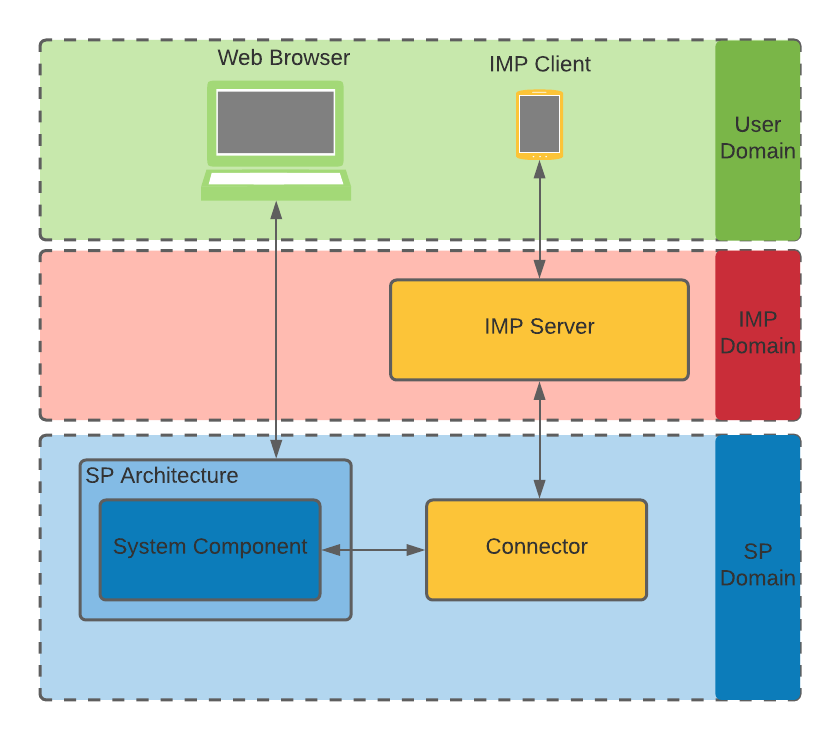
\includegraphics[scale=0.25]{Diagrams/IMP System Overview.png}
\end{figure}

The IMP system operates on three domains. The user domain contains systems, the user directly interacts with. This typically are applications on PC or smartphone and websites. The IMP system provides an application for PC and smartphone to the user for accessing IMP services. For simplification, the user is assumed to use only one device which eliminates the need for synchronization of devices. The client enables the user to manage attributes of his identity, to establish relationships, to manage relationships and to interact through relationships. 

The IMP domain contains all systems hosted by the identity management provider. In this case, the domain contains only the IMP server. The IMP server is able to communicate with IMP client and IMP connector.

The service provider domain contains the system architecture of the service provider and the IMP connector. The IMP connector contains a REST API which enables the system architecture to access IMP services.

\begin{figure}[h]
\caption{IMP System Operation Layers}
    \centering
    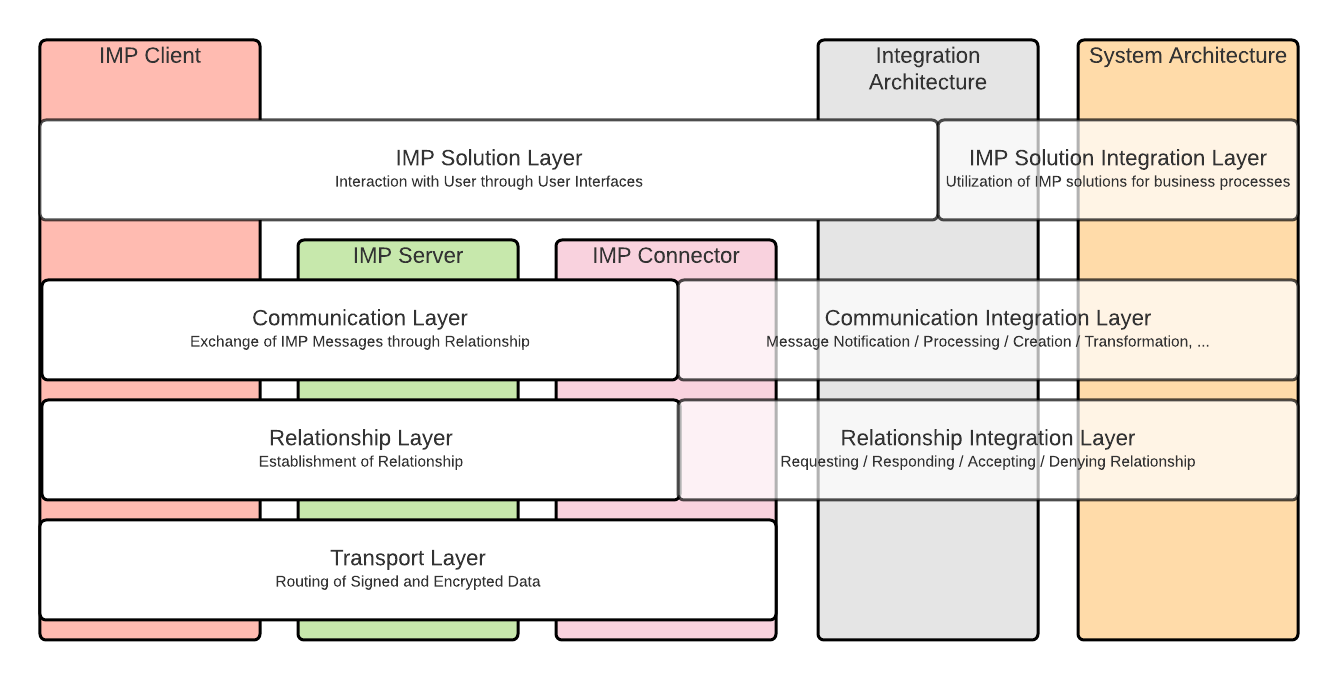
\includegraphics[scale=0.3]{Diagrams/IMP Layer Diagram.png}
\end{figure}

The operation of IMP systems can be separated in multiple layers. The layers build upon each other (from bottom to top) and provide an increasingly abstract perspective on the functionalities of each component.

\paragraph{Transport Layer}

The "transport layer" is responsible for securely routing data between IMP client, IMP server and IMP connector. Depending on the use case, the transport layer encrypts data so that it is only visible for client and connector. In this layer, IMP client and IMP connector are endpoints where data can be encrypted, decrypted, sent and received. In this layer, the IMP server is the routing component which forwards sent data to its correct destination while checking validity of messages.

\paragraph{Relationship Layer}

The "relationship layer" is responsible for establishing a relationship between IMP client and IMP connector. IMP client and IMP connector send relationship requests and responses and store relationships. The IMP server creates, stores and updates relationships and synchronizes their status with client and connector.

\paragraph{Communication Layer}

The "communication layer" is responsible for exchanging IMP messages as part of an active relationship between IMP client and IMP connector. The client can create, send, receive, process and display a list of IMP messages he is able to understand. The IMP connector is able to send and receive IMP messages through a relationship without being aware of its content. The IMP server stores an encrypted backup of all messages.

\paragraph{IMP Solution Layer}

The "IMP solution layer" is responsible for providing user interaction capabilities for construction of IMP solutions. A service provider can interact with the user in multiple ways through user interfaces of the IMP client. Depending on the use case of the service provider, interactions through the UIs can have different purposes.

For example, a service provider can decide to use relationships as a way to receive product or subscription orders. Another possibility would be to use relationships for filling in a form as part of a survey.

The user interface described in the following are a minimal example which fulfill basic requirements for establishing relationships and displaying IMP messages. An identity management provider can add multiple more specialized UIs to the application.

\begin{figure}[h]
\caption{User Application Interfaces}
    \centering
    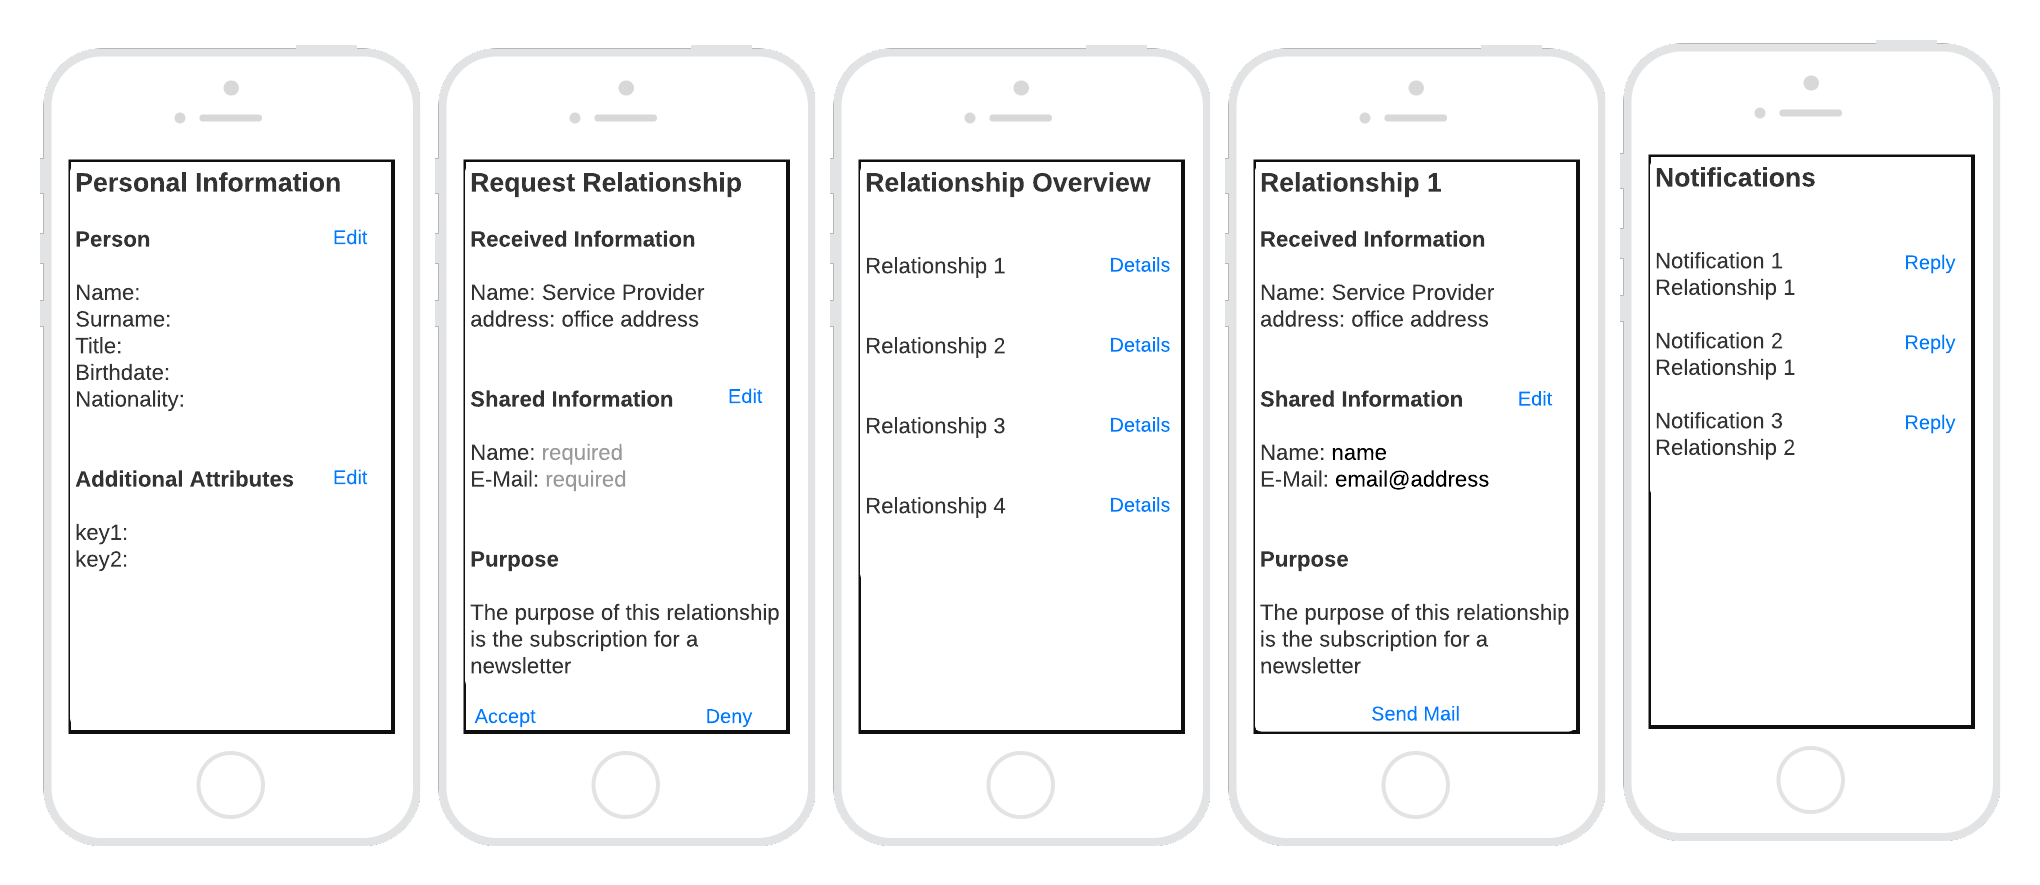
\includegraphics[scale=0.2]{Diagrams/UI.png}
\end{figure}

\paragraph{Personal Information} The attributes interface enables the user to manage attributes for his identity by adding, updating or removing values for common keys like name, surname, birth date and more. Here, the user can also create, update or delete new key-value pairs.

\paragraph{Relationship Request} On the relationship request interface, the user can scan a QR code containing a relationship template and request a corresponding relationship. The attributes required for the relationship are automatically filled in if they exist for the identity. Otherwise the user can manually enter the correct values. If all requested attributes are filled in, the user can request the relationship

\paragraph{Relationship Overview} On the relationship overview interface, the user can see all active relationships

\paragraph{Relationship Details} On the relationship details interface, the user can view the content of a relationship and change shared attributes. However, an attribute will only be changed after the service provider accepted. The user can also send a mail to the other party of the relationship.

\paragraph{Notifications} On the notifications interface, the user sees all received mails and the corresponding relationship. The user is able to reply to the mails.

\subsection{IMP Use Cases}

In this section the most important use cases of the IMP system are described in more detail.

\subsubsection{Establish Relationship}

The first step towards a relationship usually is the interest of a user. A user for example wants to subscribe to the newsletter of a service provider. The service provider needs personal information of the user to be able to send him personalized mails. To obtain the necessary attributes and receive the approval of the user, the service provider requires an established relationship.

\begin{figure}[h]
    \centering
    \caption{IMP Use Case Establish Relationship Sequence Diagram}
    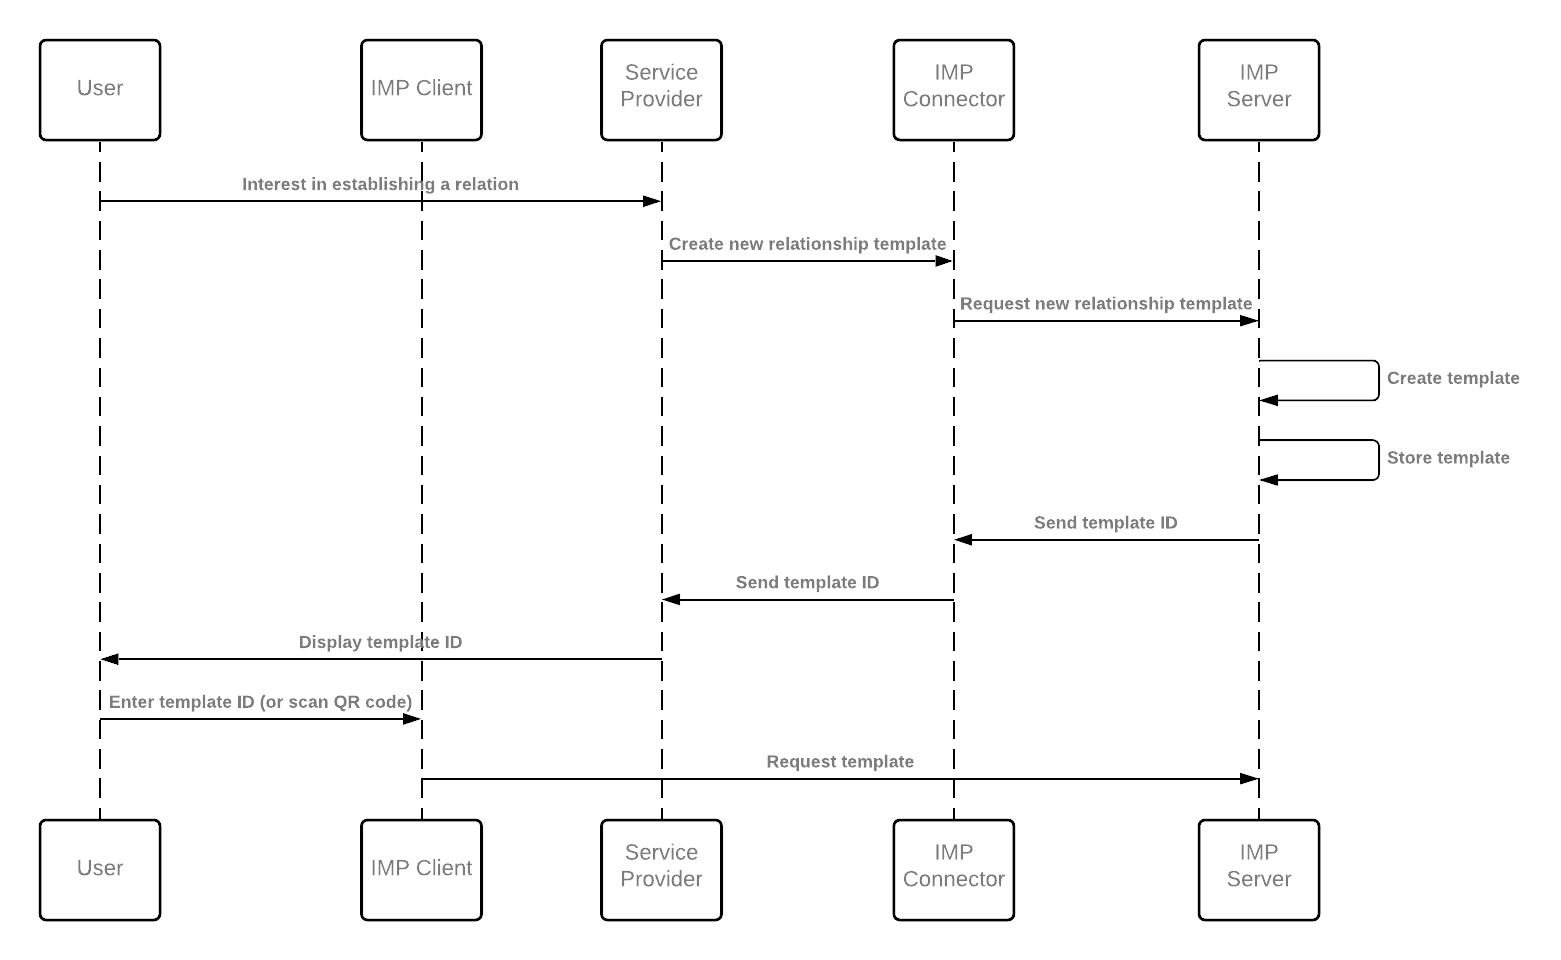
\includegraphics[scale=0.3]{Diagrams/IMP Use Case Establish Relationship Sequence Diagram 1.png}
\end{figure}

To enable users to request a relationship with the purpose of subscribing for a newsletter, the service provider has to create a relationship template. Through the REST interface of the connector, he sends a request for a new relationship template. The request contains parameters specifying the content of the relationship template. In this case, the relationship template could be configured as follows:

\begin{itemize}
    \item Title: Subscribe to the newsletter
    \item Requested Attributes: Name, Surname, E-Mail address, Interests
    \item Shared Attributes: SP Name, SP address, SP phone number, SP E-Mail address
    \item Purpose: By accepting this relationship, you agree to receive personalized mails to the shared address. Name, surname and interests are required to personalize the content of the mails.
    \item Attachments: Some legal document
\end{itemize}

\begin{wrapfigure}{r}{0.5\textwidth}
    \centering
    \caption{Relationship Request Example}
    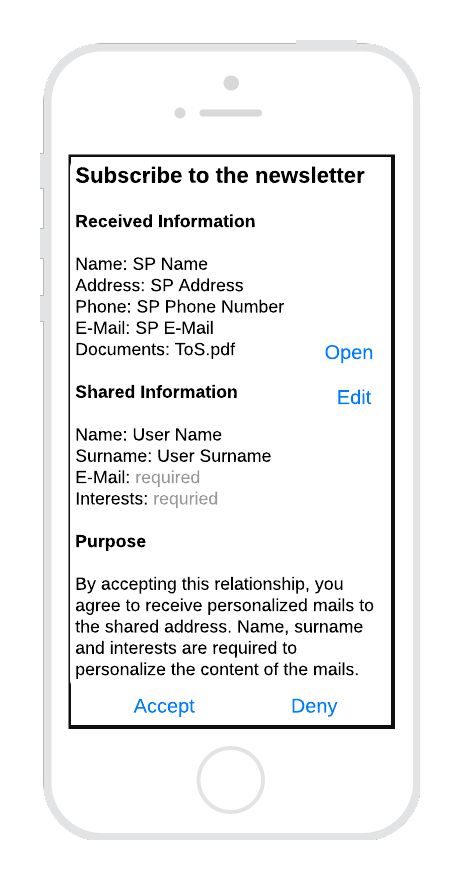
\includegraphics[scale=0.25]{Diagrams/Relationship Request Example.png}
\end{wrapfigure}

Based on the parameters of the request, the connector creates a relationship template and sends it to the IMP server. The server stores the template and returns a relationship template ID. Through this ID, the corresponding template can be retrieved from the IMP server.
The service provider can transmit the template ID to any user who wishes to subscribe for a newsletter. This can be done by for example rendering the template ID as a QR code on a website.
If the QR code is displayed to the user, he can scan it using the IMP client. The client understands that the content of the QR code contains a relationship template ID and retrieves the corresponding template from the IMP server.

The IMP client displays the relationship template to the user and automatically fills in as many requested attributes as possible.

The user can now decide if he wants to accept the relationship and share the requested attributes. If he accepts, IMP client sends a relationship request to the IMP server. The request contains all information of the relationship template in addition to the shared attributes of the user.

\begin{figure}[h]
    \centering
    \caption{IMP Use Case Establish Relationship Sequence Diagram}
    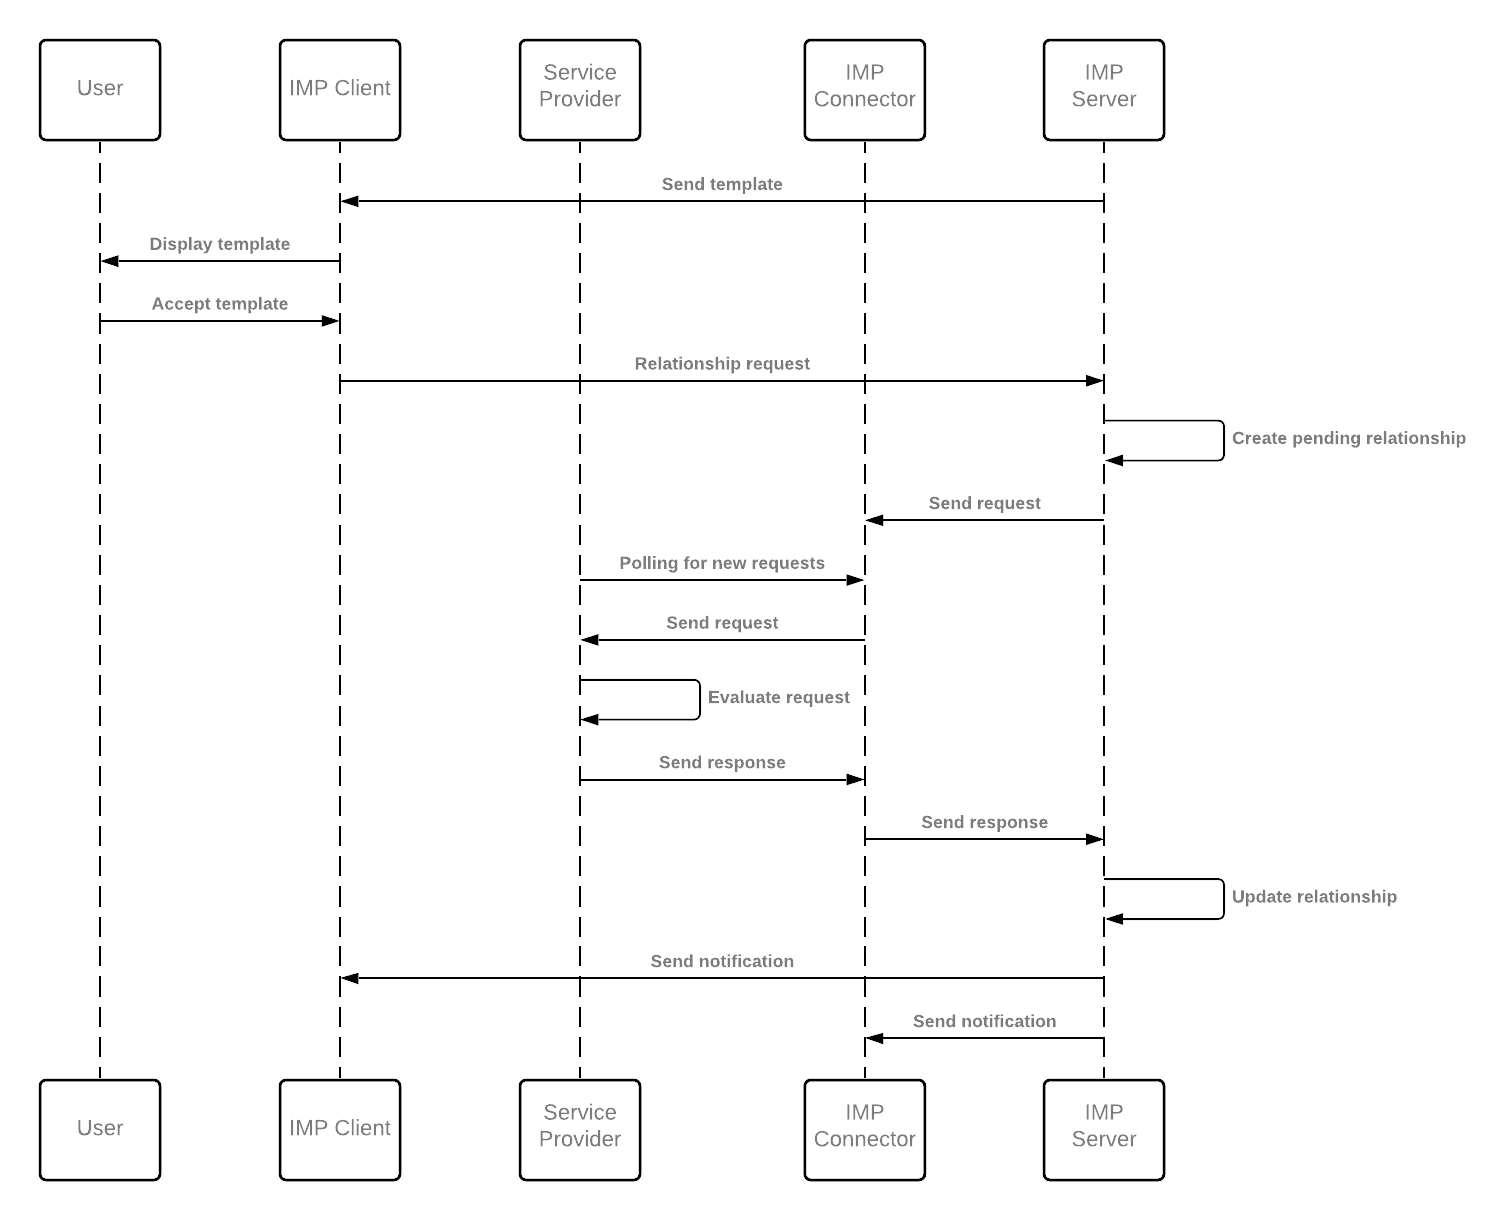
\includegraphics[scale=0.3]{Diagrams/IMP Use Case Establish Relationship Sequence Diagram 2.png}
\end{figure}

Based on the relationship request, the IMP server creates a relationship with the status "pending". A unique relationship ID is attached. The server then forwards the relationship request to the connector of the service provider.

As the system architecture of the service provider has no way of knowing when the connector receives a relationship request, he iteratively requests an update from the connector trough its REST interface. The connector responds with the received relationship request. The system architecture of the service provider processes the request in order to decide if it should be accepted. The service provider could for example verify if a relationship with the identity already exists or if the E-mail address is already registered.

The system architecture sends a relationship response to the REST interface of the connector. The response contains all information of the received relationship request with optional additional information the service provider might want to share now. This could for example be the name of the newsletter the service provider decided to select for the user based on his specified interests.

The connector sends the relationship response to the IMP server which updates the content and status of the corresponding relationship. It might be possible, that the user retracted the relationship request in the meantime. In this case, the relationship response would be dropped by the IMP server and the connector would be notified.
If however, the IMP server updates the status of the relationship to "established", both IMP client and connector are notified with the final content of the relationship.

After receiving the final relationship established notification, the system architecture of the service provider can store the shared attributes in a database along with the corresponding relationship ID for the newsletter system to access.

\subsubsection{Send Message}

Through an established message, user and service provider can exchange messages with any structure and content. However, this only makes sense if both IMP client and system architecture of the service provider can understand the messages. IMP server and IMP connector only take care of the correct routing. The list of messages an IMP client understands can be expanded by the identity management provider. It can therefore be assumed, that the IMP client understands any message service providers often want to exchange. For simplicity, in the following sections, behaviour of the IMP client for newly defined message can be defined at will. Two important types of messages were already defined: Mail Messages and Attribute Change Request-Reply Messages.

\subsubsection{Request Attribute Change}

It is possible, that in the future, the user wants to change the mail address where he receives the newsletter. As the established relationship remains to be valid, it should not be terminated, but shared attributes should be changed instead.

Through the IMP client, the user can view the corresponding relationship and edit the attributes. After he changed the mail attribute he shares, through routing by the IMP server, the IMP client sends a attribute change request message to the connector. The connector does not understand the content of the message but from which relationship it originated from. As the connector cannot notify the system architecture of the service provider, polling for new messages is required. After the system architecture receives the message, it understands the structure of the message and that the purpose of the message is an attribute change request.

The system architecture evaluates if it accepts the changes and sends a response trough the REST interface of the connector. The system architecture might execute additional processes. In this case, the mail address stored in the database would be updated.

The IMP server receives the response message through the connector and routs it to the IMP client. The IMP client understands the message, updates the value stored as part of the relationship and displays a notification to the user.

\begin{figure}[h]
    \centering
    \caption{IMP Use Case Change Relationship Attribute Sequence Diagram}
    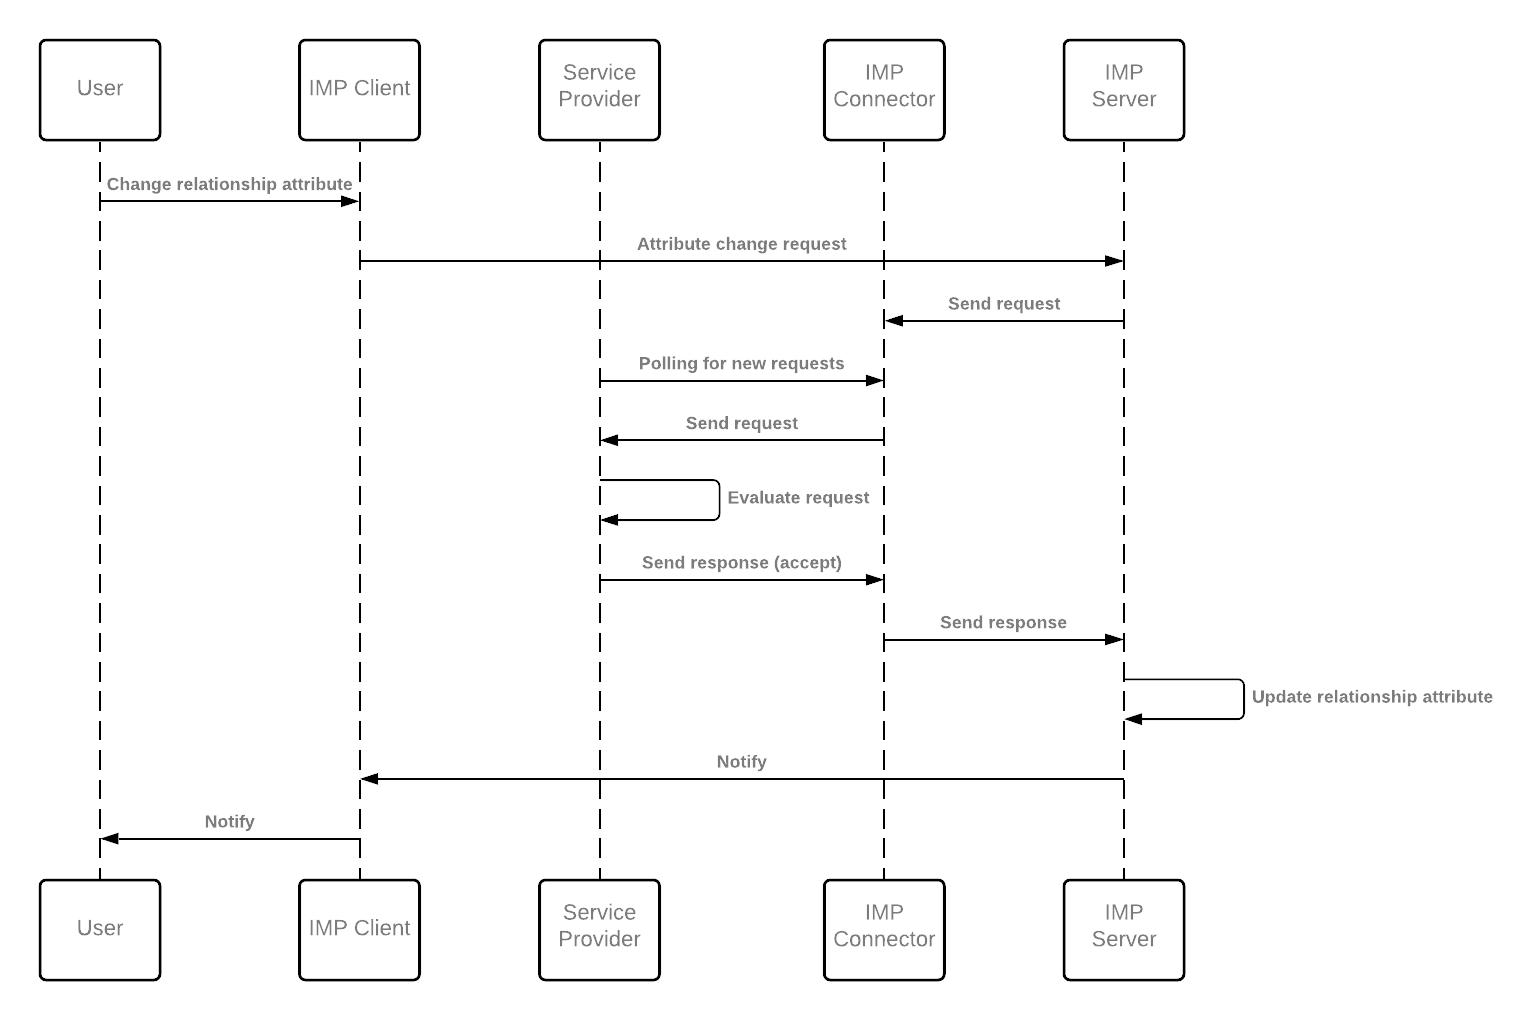
\includegraphics[scale=0.3]{Diagrams/IMP Use Case Change Realtionship Attribute Sequence Diagram.png}
\end{figure}

\subsubsection{Send Mail}

If a user has questions about the newsletter, he can send messages to the service provider as part of the relationship. Client sends the mail message to the IMP server which routes it to the connector. The system architecture polls for incoming messages. When the system architecture receives the message, it understands the content and purpose and for example notifies an employee. An employee could be notified through E-Mail and a response from the employee to the mail could automatically sent to the relationship through the REST API of the connector. Connector and IMP server route the message to the IMP client, who understands the message and displays it to the user.

\begin{figure}[h]
    \centering
    \caption{IMP Use Case Communication Sequence Diagram}
    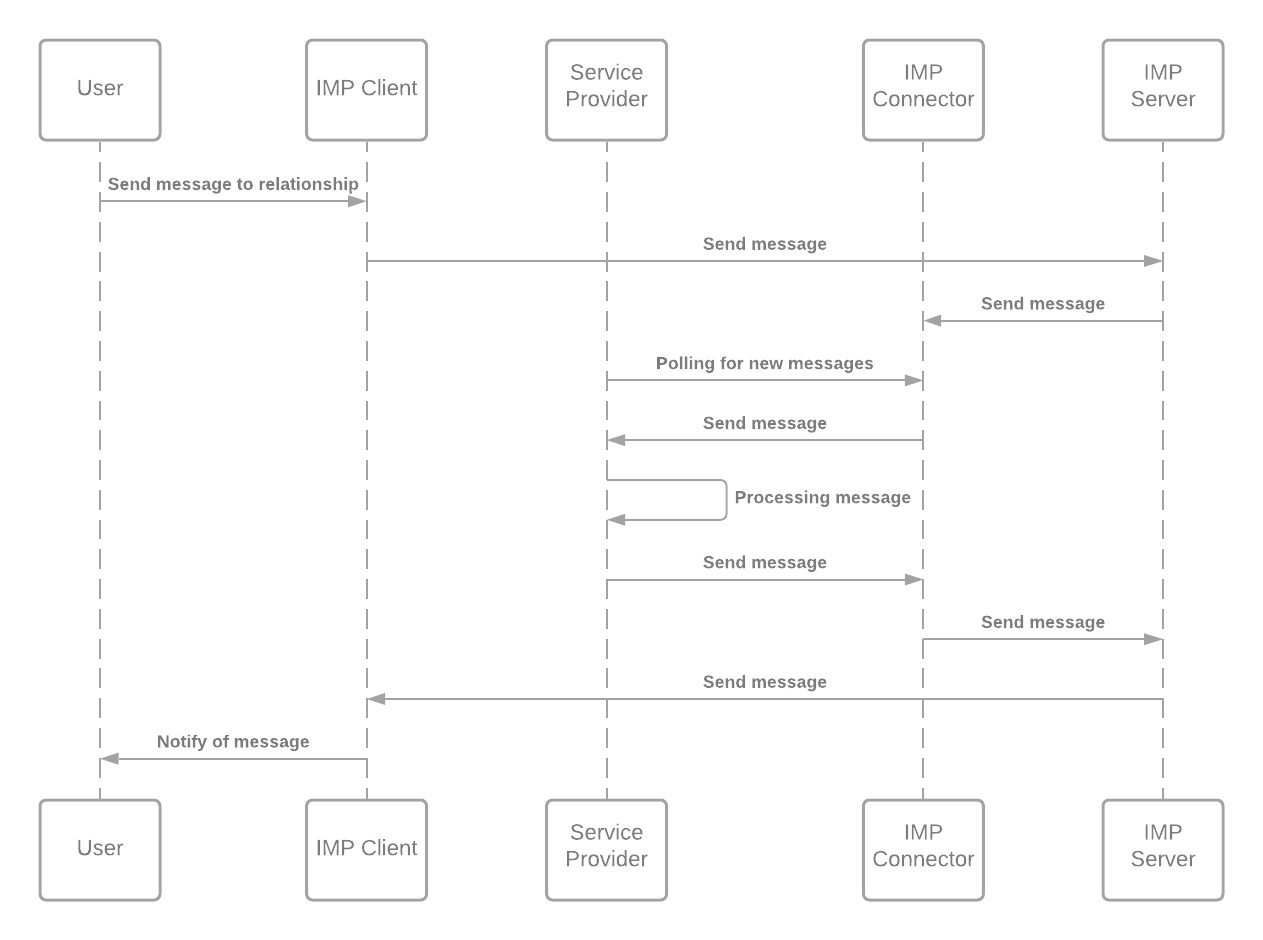
\includegraphics[scale=0.3]{Diagrams/IMP Use Case Communication Sequence Diagram.png}
\end{figure}